\documentclass[final,t]{beamer}
\mode<presentation>
  {
  \usetheme{boxes}
  }

\usepackage[orientation=landscape,size=a1,scale=1.3,debug]{beamerposter}
\usepackage{wrapfig}
\usepackage{background}
\usepackage{lipsum} % for dummy text
\usepackage{tcolorbox}
\usepackage{helvet}
\usepackage{svg}
\renewcommand{\familydefault}{\sfdefault}
\usebackgroundtemplate{\includesvg[width=\paperwidth]{template}}%
\tcbuselibrary{skins}


\title[]{\Huge\bfseries Syringe Pump for Electrochemical Cell}
\author[]{\large \textbf{Dolica Akello-Egwel} \\ \and Gary Yendell}
\date{}

% Remove Beamer Navigation Symbols
\setbeamercolor*{frametitle}{bg=}
\setbeamertemplate{navigation symbols}{}

\begin{document}

\newtcolorbox{custombox}[1]
{
  % colback=blue!10!lightgray!35!white,
  colback=white,
  arc=1mm,
  % boxsep=5mm,
  colframe=blue!70!black,
  top=3mm,
  toptitle=3mm,
  bottomtitle=3mm,
  fonttitle=\large\bfseries,
  coltitle=white,
  title=#1,
  % parbox=false,
}

\AfterEndEnvironment{custombox}{\vspace{0.6cm}}
\AfterEndEnvironment{figure}{\vspace{0.6cm}}

\begin{frame}
\maketitle
\begin{columns}[t]
  \begin{column}{.32\linewidth}
 
  \begin{custombox}{Background}
        \section{Experiment Motivation}
      Experiment requiring continuous flows, often for hours at a time.
          \textbf{Hamilton Microlab Syringe Pump}
      The Hamilton Microlab Syringe 500/600 Syringe Pump may be used for experiments that involve continuous flows through a chemical cell.\\ 
          \textbf{Existing Script \\}
      The existing script allowed simple commands, but did not provide an interface to handle complex commands involving multiple syringe moving simultaneously. Attempts at having the syringe pump run overnight were unsuccessful.
  \end{custombox}

  \begin{custombox}{Objectives}
     \begin{itemize}
        \item Make a Python library for controlling the Hamilton Microlab Syringe Pump 
        \item Add EDM screens 
        \item Add cycling ability. 
        \item Interface with EPICS. 
    \end{itemize} 
  \end{custombox}

      \begin{figure}[t]
          {%
        \setlength{\fboxsep}{0pt}%
        \setlength{\fboxrule}{3pt}%
          \fbox{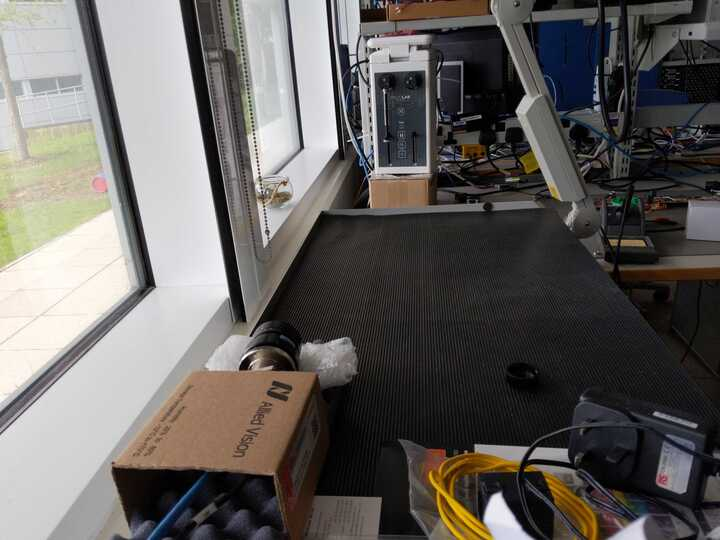
\includegraphics[width=0.7\linewidth]{images/camerasetup}}%
        }%
% \centering
      \end{figure}

  \begin{custombox}{Remote Working}
      Section about remote working setup.
  \end{custombox}
  \end{column}

 %%%%%%%%%%%%%%%%%%%%%%%%%%%%%%%%%%%%%%%%%%%%%%%%%%%%%%%%%%%


  \begin{column}{.32\linewidth}

  \begin{custombox}{Python Library}
    Discuss the Python library. 
  \end{custombox}
  
      \begin{figure}[t]
          {%
        \setlength{\fboxsep}{0pt}%
        \setlength{\fboxrule}{3pt}%
          \fbox{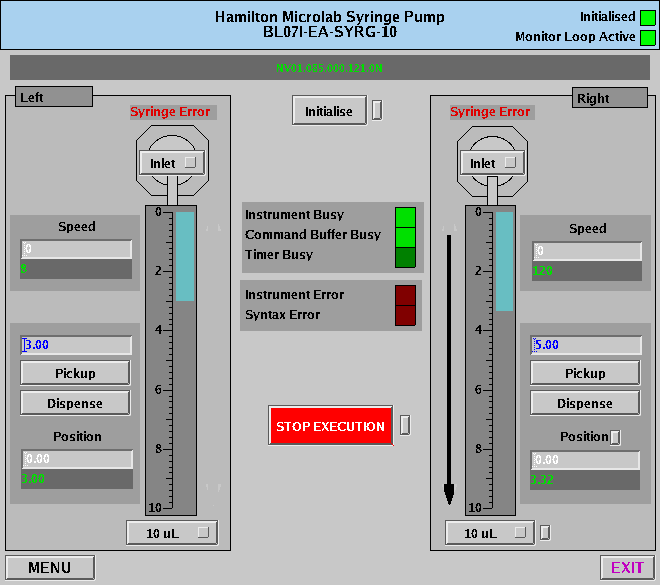
\includegraphics[width=0.8\linewidth]{images/mainscreen.png}}%
              \caption{EDM screen}
        }%
% \centering
\end{figure}

  \end{column}

  
  %%%%%%%%%%%%%%%%%%%%%%%%%%%%%%%%%%%%%%%%%%%%%%%%%%%%%%%%%%%

  \begin{column}{.32\linewidth}

      \begin{custombox}{EPICS and \texttt{softioc}}
          \begin{wrapfigure}{r}{0.3\textwidth}
      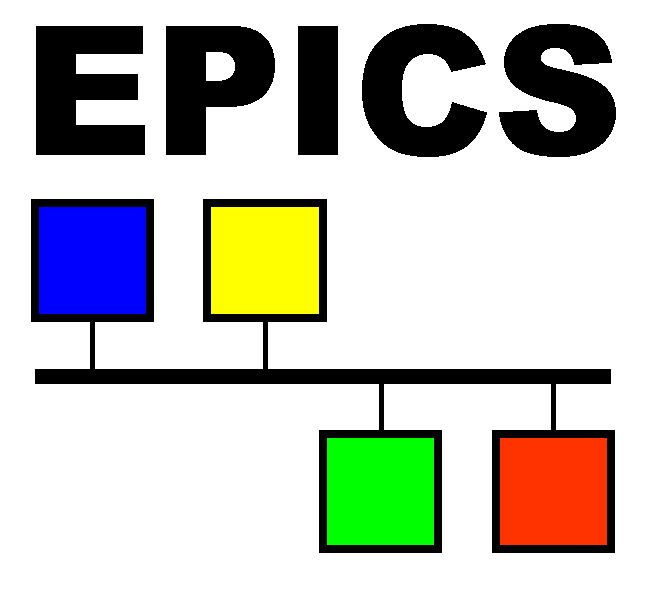
\includegraphics[width=\linewidth]{images/epicslogo}
          \end{wrapfigure}
      The Experimental Physics and Industrial Control System (EPICS) comprises a set of software components and
      tools that can be used to create distributed control systems. EPICS provides capabilities that are typically expected from a distributed control system:
  \end{custombox}

 
  \begin{custombox}{Final Thoughts}
      \textbf{Results} 
    \begin{itemize}
        \item Permanent "Syringe Error" message 
        \item Behaviour of syringe movement indicator arrows not ideal, especially for fast movements 
    \end{itemize}

      \textbf{Further Work }
    \begin{itemize}
        \item Develop a simulator for the syringe pump and use it to create system tests
        \item Add a cleaning command 
    \end{itemize}
  \end{custombox}

  \end{column}
  \end{columns}
    
\end{frame}

\end{document}
